\setcounter{chapter}{1}
% Setting Chapter 2
%  
\chapter{Quy trình thực nghiệm lọc tách \ce{^226Ra} trong đất và nước}

\section{Đôi nét về  quy trình chiết tách/lọc \ce{^226Ra} trong đất và nước ngầm}

    \subsection{Quy trình chiết tách phân đoạn BCR}

    Những năm đầu 1990, các nghiên cứu về xây dựng quy trình chiết tách phân đoạn kim loại nặng, nổi bật như Koguh và cộng sự (1994), Kozuh  và cộng sự (1996), Ure và cộng sự (1996). Mục tiêu của quy trình nhằm đánh giá khả năng hòa tan trong nước trong từng pha, và tính linh động trong môi trường, từ đó có phương pháp cụ thể để loại bỏ các kim loại nặng trong đất và trầm tích ~\cite{BCR:OrginNusa}. Mỗi quy trình lại tập trung cụ thể vào một kim loại, và hóa chất phân tích được lựa chọn có độ hoạt động hóa học cao với kim loại phân tích đó. Do đó, dữ liệu thu được của mỗi nghiên cứu không thể được so sánh, hoặc tham khảo. Năm 1987, nhằm xây dựng một quy trình chiết tách kim loại có tính tiêu chuẩn và đồng bộ, một nhóm các chuyên gia của Viện tiêu chuẩn và đo lường Châu Âu \footnote{Institute for Reference Materials and Measurements: Viện được thành lập vào năm 1957 theo Hiệp ước Rome và bắt đầu hoạt động vào năm 1960 dưới tên của Cục tiêu chuẩn đo lường Hạt nhân (CBNM). Năm 1986, Viện đổi tên thành Ủy ban về đo lường Châu Âu. Năm 1993, Viện chính thức đổi tên là Viện tiêu chuẩn về đo lường Châu Âu, tập trung về xây dựng tiêu chuẩn đo lường từ an toàn thực phẩm đến ô nhiễm môi trường, có trụ sở chính đặt tại Bỉ (Theo en.wikipedia.org)} đã đề xuất một quy trình trích xuất ba bước (BCR CRM - 601), từ dữ liệu thu được có thể xác định độ linh động của kim loại nặng  trong từng phân đoạn. ~\cite{BCR:PeterSvete}.  Quy trình BCR được áp dụng rộng rãi trong phân tích kim loại nặng trong đất, bùn, và trầm tích. Ưu điểm của quy trình, là sự thống nhất trong phân tích các kim loại nặng, và sử dụng mẫu chuẩn để phân tích, kết quả phân tích được chứng nhận tiêu chuẩn Châu Âu, và giảm thời gian phân tích. Quy trình BCR CRM-601 gồm ba phân đoạn chính:
        \begin{enumerate}[label=(\arabic*) ]
            \item Phân đoạn trao đổi ion và axit hóa: Trao đổi ion kim loại và liên kết với cacbonat.
            \item Phân đoạn khử: Liên kết của Sắt and mangan hydroxide
            \item Phân đoạn oxi-hóa: Liên kết hữu cơ và sulfua
        \end{enumerate}


    \subsection{Phương pháp hấp thụ \ce{^226Ra} bằng sợi \ce{MnO2}}

      Từ nghiên cứu của nhóm  Willard S. Moore (1973) về các đặc tính thuỷ văn hải dương như: quỹ đạo vận chuyển của khối nước biển ven bờ, sự pha trộn theo chiều đứng và chiều ngang của nước gần bờ với nước đại dương, tốc độ bổ cấp nước ngầm... sử dụng  hai đồng vị có thời gian bán rã dài là \ce{^226Ra} và \ce{^228Ra} có sử dụng làm  đồng vị đánh dấu và chỉ thị môi trường ~\cite{MnO2:Moore} . Trong quá trình nghiên cứu, nhóm đã xây dựng và phát triển phương pháp hấp thụ \ce{^226Ra} trong nước bằng sợi acrylic tẩm mangan oxit.
      
      Các kết quả phân tích , nhóm Willard S. Moore đã nhận xét rằng: 
      \begin{itemize}
        \item Phương pháp đồng kết tủa radium với \ce{BaSO4}, không phù hợp để tạo sợi lọc nước biển. 
        \item \ce{MnO2/Mn(OH)2} hấp thụ \ce{^226Ra} tốt so với sắt oxit của nhóm nhóm Krishnaswami (1972). Cụ thể, phương pháp lọc bằng sợi mangan oxit có hiệu suất lọc \ce{^226Ra} trên 90\% từ 170L nước biển, với tốc độ dòng chảy 400 cm/phút, trong khi sợi Sắt oxit chỉ có hiệu suất lọc khoảng 11\%.
        \item  Nhóm đã đề xuất cải tiến phương pháp bằng tẩm sợi acrylic với các muối \ce{MnCO3}, \ce{FeS}, và \ce{MnS}, có thể tăng hiệu suất lọc radium. Bên cạnh đó, muối Zirconium (\ce{[OH]^-}, \ce{[PO4] ^{3-}} và   \ce{[Mo4]^{2-}}) có hiệu suất hấp thụ radium cao nhất, nhưng chi phí của Zirconium khá cao, không phù hợp để lọc thể tích mẫu nước biển (từ 1L trở lên). 
    \end{itemize}
    
    Dựa trên thành công của phương pháp lọc \ce{^226Ra} bằng sợi acrylic tẩm \ce{MnO2} của nhóm Willard S. Moore (1973), tác giả  cải tiến  phương pháp sử dụng sợi tổng hợp tẩm   \ce{MnO2} thay vì sử dụng sợi acrylic tẩm \ce{MnO2}. 




    % TODO: --------------------------------------------------------------------

\section{Hệ thiết bị RAD7}
\label{section:HeThietBiRAD7}

Hệ thiết bị  RAD7,  là thiết bị chuyên sử dụng để đo khí \ce{^222Rn} và \ce{^220Rn} hoàn chỉnh, đáp ứng nhiều mục đích sử dụng khác nhau. Hệ thiết bị RA7 đi kèm các phụ kiện như ~\cite{Thesis:HNPThu}: 
    \begin{itemize}
        \item Các lọ chứa    mẫu nước đo dung tích 250 mL và 40 mL.
        \item Bộ phận thu khí radon trong nước gồm: khối ba đầu làm bằng kim loại
        không gỉ, ống nhựa đôi dùng để giữ khối ba đầu, ống đệm bằng vật liệu tổng hợp, đầu sục khí.
        \item Ống chứa than hoạt tính.
        \item Các đầu lọc khí và ống dẫn khí từ ngoài vào RAD7 và từ RAD7 ra ngoài.
    \end{itemize} 
    


    Sơ đồ hệ thí nghiệm đo nồng độ radon để xác định hàm lượng \ce{^226Ra} đã lọc tách chứa trong phần mẫu lỏng  được thể hiện trên hình ~\ref{figure:SoDoLayRnRD7}. Khi bắt đầu quá trình đo, bơm trong RAD7 sục khí vào lọ đựng mẫu, đẩy khí phóng xạ hòa tan trong lọ ra khỏi nước và tạo thành dòng lưu thông khép kín đi qua buồng đo. Hiệu suất tách radon khỏi nước, đưa vào vòng không khí khoảng 94\% đối với lọ 250 ml. Radon thoát khỏi mẫu nước, liên tục tuần hoàn qua ống hút ẩm, buồng đo và sau đó trở về mẫu nước để thiết lập trạng thái cân bằng giữa radon trong nước và không khí. Sau 5 phút, bơm trong RAD7 sẽ dừng hoạt động. Ngắt kết nối giữa mẫu và RAD7, hệ thiết bị được đóng kín và hoạt động đo trong 4 đến 5 giờ. 


    
    \begin{figure}[htbp]
        \centering
        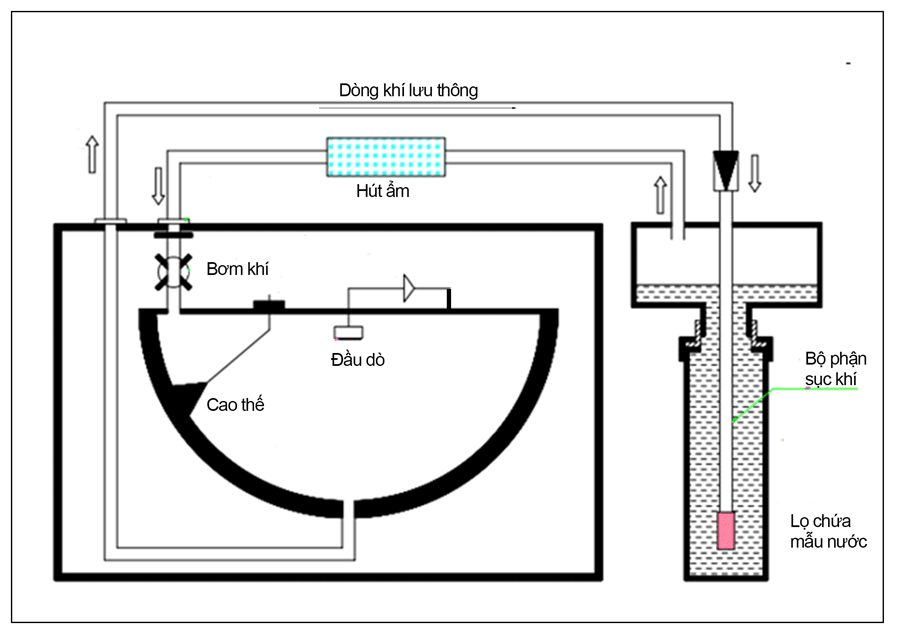
\includegraphics[width=0.75\textwidth]{Image/MnO2-Figure7.png}
        \caption{Sơ đồ lấy khí radon trong mẫu nước và đo bằng RAD7}
        \label{figure:SoDoLayRnRD7}
    \end{figure}



    \textbf{Nguyên lý xác định nồng độ radon của RAD7} ~\cite{Thesis:HNPThu}: 
    
    Buồng đo khí phóng xạ bên trong RAD7 có hình bán cầu, được phủ phía trong một lớp dẫn điện. Bộ phận ghi nhận tín hiệu làm bằng tấm silicon phẳng và được đặt ở tâm bán cầu. Mạch điện cung cấp điện áp (2000 - 2500) V, tạo nên điện trường trong toàn bộ buồng đo. Điện trường giúp đẩy các hạt tích điện đến đầu dò. RAD7 xác định nồng độ radon dựa vào việc đo phổ năng lượng của tia alpha. Khi bắt đầu quá trình đo, máy bơm đưa khí chứa radon (đã được làm khô) vào buồng. Đầu lọc khí chỉ cho khí hiếm đi qua và ngăn cản các đồng vị con cháu gây ảnh hưởng đến kết quả đo. Radon là nguyên tử khí trung hòa về điện nên không được hệ đo ghi nhận cho đến khi phân rã, tạo thành \ce{^218Po}, tồn tại dạng ion dương. Điện trường trong buồng đo mang các hạt tích điện dương đến đầu dò. \ce{^218Po} phân rã ngay trên bề mặt đầu dò. Hạt alpha tạo ra có khả năng đập vào đầu dò và tạo nên xung điện có độ lớn tỷ lệ thuận với năng lượng. Các quá trình phân rã tiếp tục diễn ra tạo thành các hạt alpha có năng lượng khác nhau, sinh ra các tín hiệu có biên độ khác nhau, được khuếch đại và chuyển thành tín hiệu số nhờ các mạch điện. Bộ xử lý thu nhận các tín hiệu, lưu trữ trong bộ nhớ theo năng lượng của từng hạt alpha và xây dựng các đỉnh phổ năng lượng riêng biệt. Số đếm ở các cửa sổ A (\ce{^218Po}) và C (\ce{^214Po}) để xác định nồng độ radon vì chúng ghi nhận alpha từ phân rã của các con cháu radon. Số đếm ở các cửa số B (\ce{^216Po}) và D (\ce{^212Po}) được ghi nhận để xác định nồng độ thoron vì chúng chứa số đếm từ các con cháu của thoron. Hình ~\ref{figure:PhoAlphaRAD7} minh họa ví dụ một phổ alpha lấy từ RAD7. Thông thường, khoảng sau 3 giờ, số đếm ở cửa sổ C sẽ cân bằng với số đếm ở cửa sổ A. Vì vậy, 3 giờ đầu, nồng độ radon sẽ được xác định dựa vào số đếm ở cửa sổ A, sau đó, cả số đếm ở cửa sổ A và cửa sổ C đều được dùng để xác định nồng độ radon . Ngoài ra, RAD7 gộp các tín hiệu nhiễu và số đếm alpha ghi nhận được từ đồng vị \ce{^210Po} vào cửa sổ O. \ce{^210Po} là đồng vị con cháu của radon xuất hiện khi máy được sử dụng trong một thời gian dài. Các số đếm này không đóng góp vào nồng độ radon vì đã được đưa vào một cửa sổ khác. Đây là điểm ưu việt của RAD7.


    \begin{figure}[htbp]
        \centering
        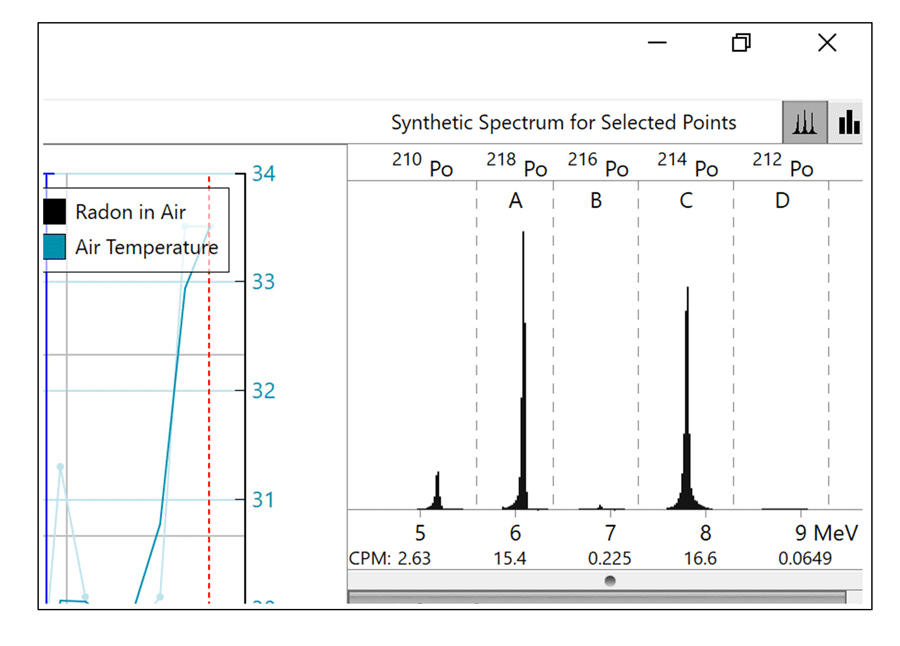
\includegraphics[width=0.68\textwidth]{Image/MnO2-Figure2.png}
        \caption{Phổ alpha lấy từ RAD7}
        \label{figure:PhoAlphaRAD7}
    \end{figure}
    

    \textbf{Đo nồng độ \ce{^222Rn} trong mẫu nước bằng hệ thiết bị RAD7}

\begin{itemize}
    \item Trên màn hình hiển thị của RAD7, chọn mục Setup thiết lập các chế độ đo.
    \item Tại cửa Inlet, ta thực hiện nối máy với ống hút ẩm qua đầu lọc và dây dẫn khí,  đầu còn lại của ống được nối vào bộ phận thu khí từ lọ nước.
    \item Tại cửa Outlet của RAD7, ta thực hiện nối bộ phận thu khí từ lọ nước.
    \item Để tiến hành đo, ta thực hiện: chọn Test, chọn Start và chọn Enter để bắt đầu quá trình đo.
    \item Khi hết thời gian đo, máy sẽ tự động dừng. Trong trường hợp gặp phải sự cố, để dừng đo tức thời, ta thực hiện, chọn Test, rồi chọn Stop 
    \item Làm sạch máy.
    \item Lấy số liệu: Khi đo xong, kết quả có thể được xuất ra máy in hoặc chuyển sang máy tính
    nhờ dây cáp nối máy tính - RAD7 và phần mềm CAPTURE.
\end{itemize}

 
    % FIX Lai hinh DigramRAD7
    \begin{figure}[htbp]
        \centering 
        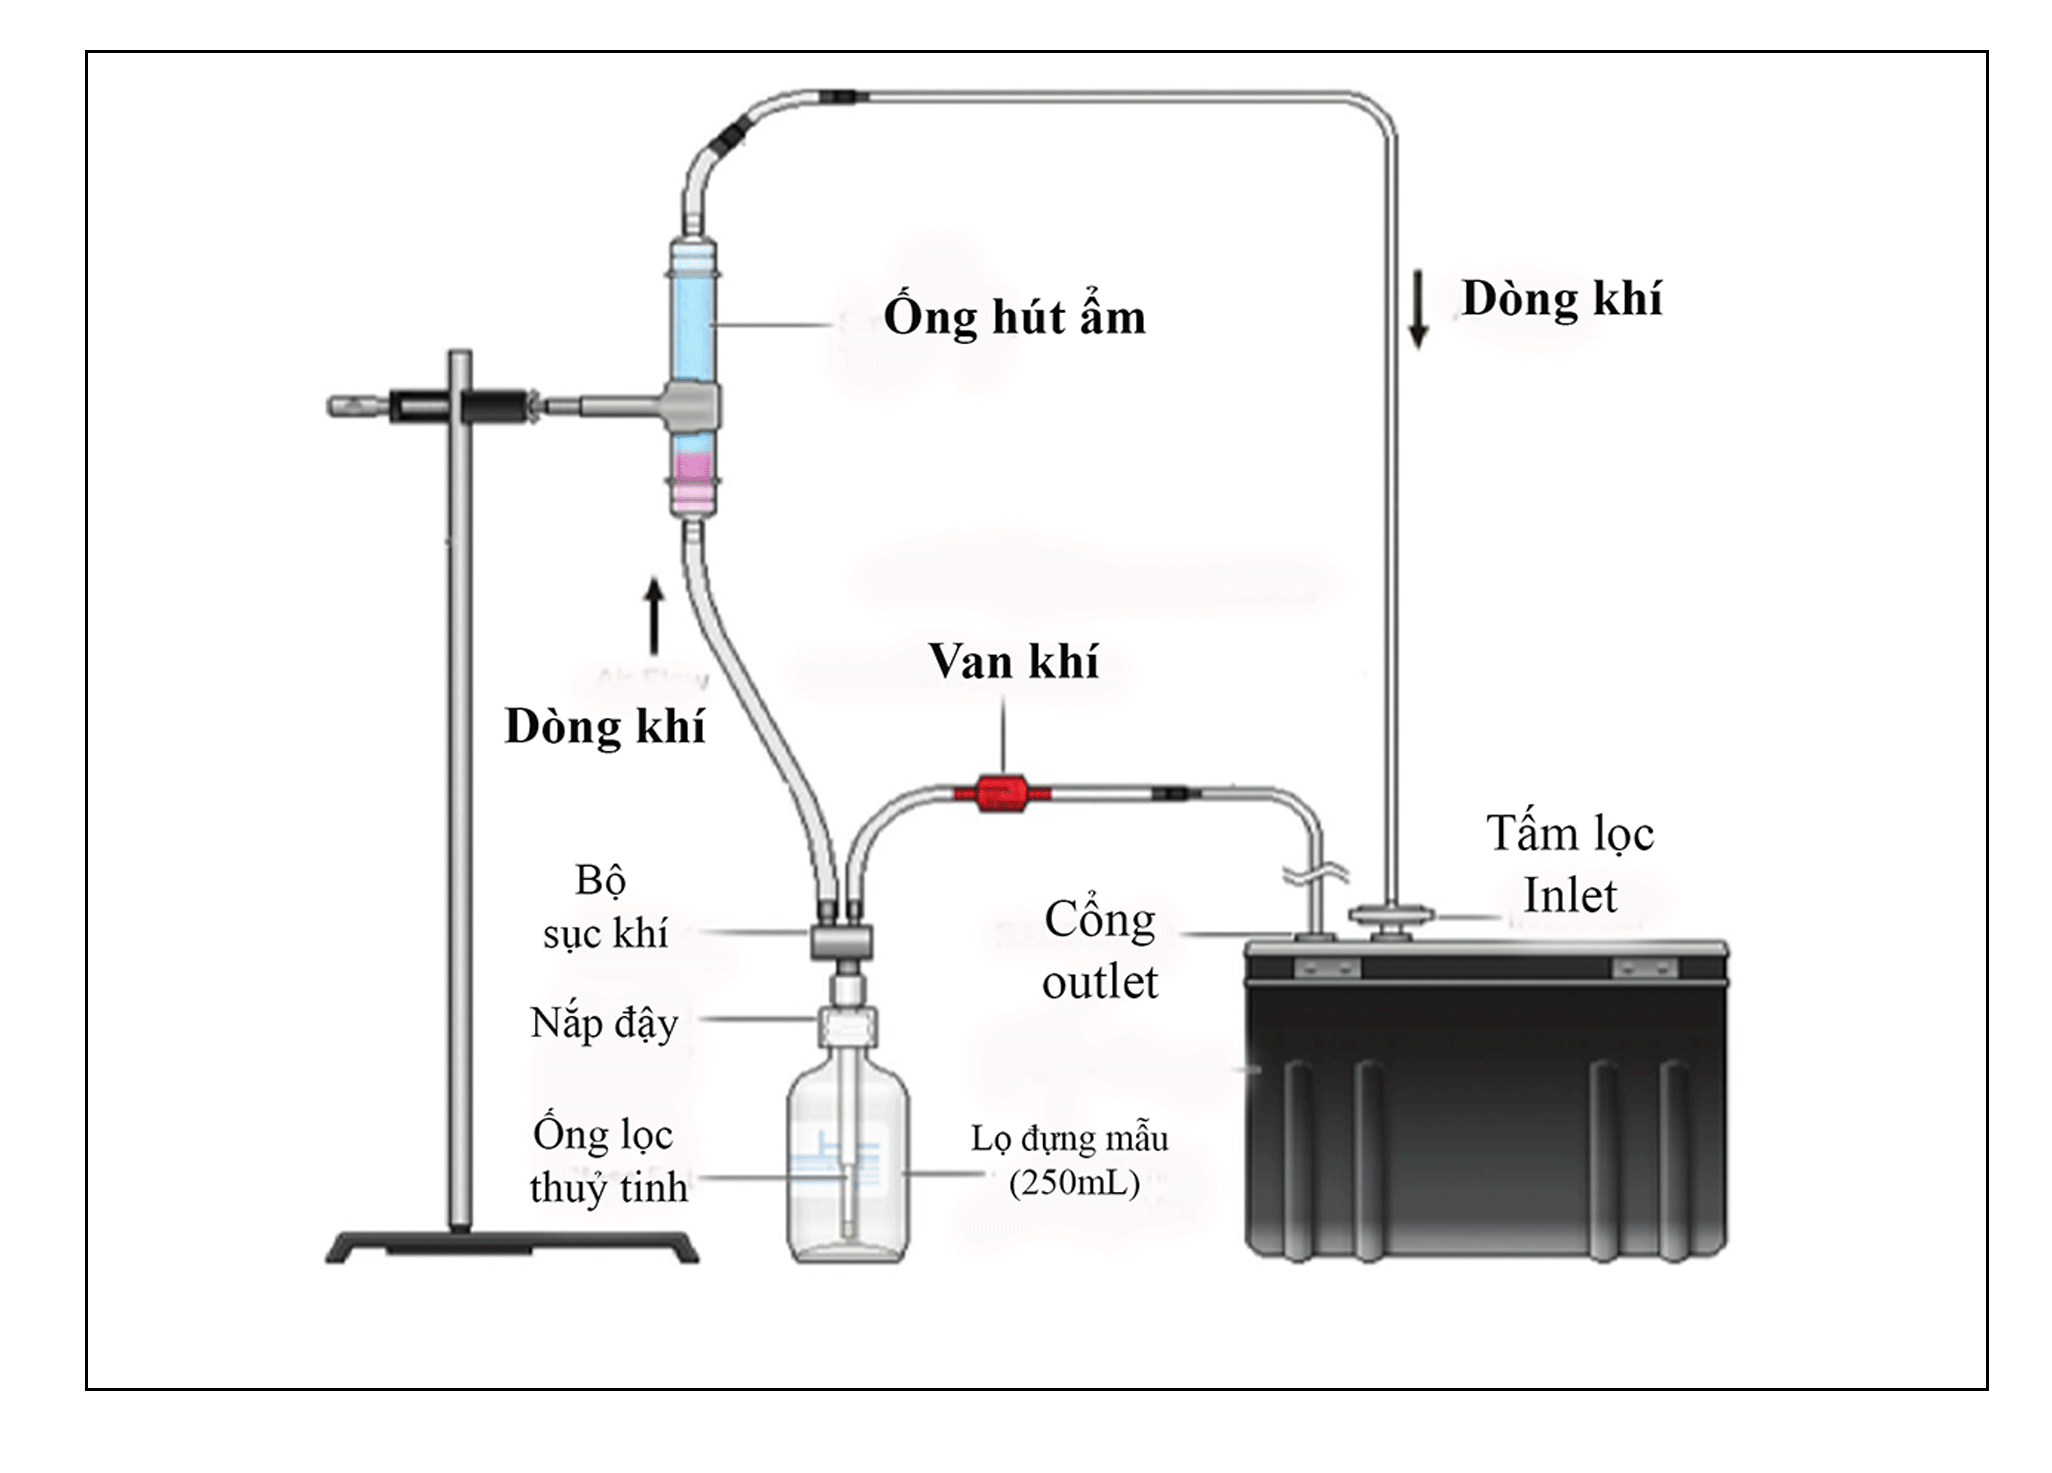
\includegraphics[width=0.75\textwidth]{Image/MnO2-Figure1.png}
        \caption{Sơ đồ bố trí đo khí \ce{^222Rn} của mẫu nước bằng hệ thiết bị RAD7}
        \label{figure:RADSoDoDoMauNuoc}
    \end{figure}



        % TODO: BCR ------------------------------------------
        \subsection{Xác định nồng độ \ce{^226Ra} chiết tách được sau mỗi phân đoạn của  quy trình BCR}
    Mẫu nước được tách ra sau khi li tâm ở mỗi phân đoạn được nhốt trong vòng 10 ngày. Trong thời gian này,  \ce{^226Ra} tồn tại trong nước phân rã alpha đồng vị \ce{^222Rn}. Khi lượng \ce{^222Rn} sinh ra đủ lớn, ta tiến hành đo nồng độ \ce{^222Rn} trong nước bằng thiết bị RAD7.    Hàm lượng \ce{^226Ra} trong phần lỏng thu được qua mỗi bước chiết tách được xác định gián tiếp thông qua nồng độ \ce{^222Rn} theo công thức ~\ref{equationBCR:RntoRa}: 
    
    \begin{equation}
        C_{Ra} = \dfrac{k.C_{Rn}.V}{\qty(1-e^{-\lambda.t})m}
        \label{equationBCR:RntoRa}
    \end{equation}
    
    
    Sai số kết quả được xác định theo công thức ~\ref{equationBCR:SigmaRntoRa}. 
    \begin{equation}
        \sigma_{C_{Ra}} = C_{Ra}.\sqrt{\qty(\dfrac{\sigma_{Rn}}{C_{Rn}})^2 + \qty(\dfrac{\sigma_{k}}{k})^2 }
        \label{equationBCR:SigmaRntoRa}
    \end{equation}
    
    
    Trong đó:
    \begin{itemize}
    \item  $C_{Rn} \pm \sigma_{C_{Rn}}$  (Bq/L) là nồng độ phóng xạ của \ce{^222Rn} trong 250 ml dung dịch mẫu và sai số;  V = 250 (mL) là thể tích dung dịch mẫu; Khối lượng mẫu đất đem phân tích, m = 10 g.
    \item $C_{Ra} \pm \sigma_{C_{Ra}}$ (Bq/kg) là nồng độ phóng xạ của \ce{^226Ra} trong phần lỏng sau khi lọc tách trong mỗi bước của mẫu cần phân tích và sai số;
    \item Thời gian nhốt t = 10 ngày; Hằng số phân rã của \ce{^222Rn} = $0.2621 (\text{ngày}^{-1})$
    \item Hệ số k là hệ số hiệu chỉnh sự thất thoát radon trong quá trình nhốt mẫu. Hệ số k được xác định bằng cách sử dụng nguồn chuẩn \ce{^226Ra} hoạt độ xấp xỉ 5 Bq của NIST. Nguồn được nhốt 10 ngày trong lọ chuyên dụng của RAD7 chứa 250 ml nước cất. Hệ số k là tỷ số giữa hoạt độ được cung cấp bởi nhà sản xuất và hoạt độ đo được bằng RAD7. Hệ số k được xác định trung bình qua 5 lần nhốt mẫu và đo. Hệ số trung bình đạt $1,25 \pm 0,03$ ~\cite{Thesis:HNPThu}. 
    
    \end{itemize}
    
    % TODO: ------------------------ MnO2


    \subsection{Xác định nồng độ \ce{^226Ra} trước và sau khi thực hiện phương pháp hấp thụ \ce{MnO2}}

    Mẫu nước trước và sau khi lọc tách bằng phương pháp hấp thụ \ce{^226Ra} trên sợi tổng hợp, sẽ được nhốt trong lọ kín 250 ml trong 10 ngày. Sau đó, nồng độ \ce{^226Ra} được xác định bằng hệ thiết bị RAD7,  từ công thức (~\ref{equation:RntoRa}), ta có thể suy ra nồng độ \ce{^226Ra}  trong mẫu nước.

        \begin{equation}
            C_{Ra} = \dfrac{k.C_{Rn}}{\qty(1-e^{-\lambda.t})}
            \label{equation:RntoRa}
        \end{equation}

        \begin{equation}
            \sigma_{Ra} = C_{Ra}.\sqrt{\qty(\dfrac{\sigma_{Rn}}{C_{Rn}})^2 + \qty(\dfrac{\sigma_{k}}{k})^2 }
        \end{equation}

Trong đó:
\begin{itemize}
    \item  $C_{Rn} \pm \sigma_{C_{Rn}}$  (Bq/L) là nồng độ phóng xạ của \ce{^222Rn} trong 250 ml dung dịch mẫu;  V = 250 (mL)
    \item $C_{Ra} \pm \sigma_{C_{Ra}}$ (Bq/L) là nồng độ phóng xạ của \ce{^226Ra} trong phần lỏng sau khi lọc tách  của mẫu cần phân tích;
    \item Thời gian nhốt t = 10 ngày; Hằng số phân rã của \ce{^222Rn} = $0.2621 (\text{ngày}^{-1})$
    \item Hệ số k là hệ số hiệu chỉnh sự thất thoát radon trong quá trình nhốt mẫu. Hệ số k được xác định bằng cách sử dụng nguồn chuẩn \ce{^226Ra} hoạt độ xấp xỉ 5 Bq của NIST. Nguồn được nhốt 10 ngày trong lọ chuyên dụng của RAD7 chứa 250 ml nước cất. Hệ số k là tỷ số giữa hoạt độ được cung cấp bởi nhà sản xuất và hoạt độ đo được bằng RAD7. Hệ số k được xác định trung bình qua 5 lần nhốt mẫu và đo. Hệ số trung bình đạt $1,25 \pm 0,03$ ~\cite{Thesis:HNPThu}. 
    
\end{itemize}

    

\section{ Quy trình thực nghiệm lọc tách \ce{^226Ra} trong đất}
Quy trình lọc tách \ce{^226Ra} được áp dụng trên một số mẫu đất được thu thập tại khu vực Ninh Sơn, tỉnh Ninh Thuận. Khu vực này có một số mẫu đất chứa hàm lượng phóng xạ \ce{^226Ra} cao trên mức trung bình trên thế giới theo UNSCEAR (Thu, 2019).

%    FIXME: Thu,2019 là gì


\subsection{Xác định hàm lượng \ce{^226Ra} trong đất}

    \textbf{Chuẩn bị mẫu đất} 

    \begin{itemize}
        \item Mẫu đất tại hiện trường được lấy ở độ sâu từ 20 – 30 cm. Sau khi được di chuyển về phòng thí nghiệm, mẫu được hong khô, nhặt sạch các dị vật: sỏi đá, rác. 
        \item   Mẫu đất khô được nghiền nhỏ, rây qua rây có đường kính lỗ 0,2 mm để đảm bảo mẫu được đồng nhất. Tiếp tục sấy mẫu ở nhiệt độ 105 (độ C) trong 8 (giờ) và đóng mẫu vào hộp trụ. Lưu ý mẫu cần được đóng đồng đều, chiều cao khoảng 2 cm, đảm bảo độ kín của hộp tốt nhất có thể.
        \item  Nhốt mẫu ít nhất 30 ngày để tạo cân bằng phóng xạ giữa \ce{^226Ra} và các đồng vị con cháu trước khi đo bằng hệ phổ kế gamma.
    \end{itemize}



    
    \textbf{Xác định hàm lượng \ce{^226Ra} bằng hệ phổ kế gamma}
   
    Hệ thiết bị được sử dụng để phân tích hàm lượng phóng xạ \ce{^226Ra} trong khóa luận là phổ kế gamma GC3520 của hãng Canberra, đặt tại Phòng thí nghiệm Kỹ thuật Hạt nhân. Hệ đo được thiết lập để ghi nhận bức xạ gamma với khoảng năng lượng từ 40 keV đến 3 MeV. 

    Hệ đo gồm các thiết bị: đầu dò và nguồn nuôi cao thế cho đầu dò, bộ phận khuếch đại và tiền khuếch đại, bộ phân tích đa kênh, buồng chì che chắn phông bao quanh đầu dò và nguồn, thiết bị làm lạnh cho đầu dò. Đầu dò HPGe có độ phân giải năng lượng và hiệu suất ghi tương đối tại đỉnh phổ có năng lượng 1332 keV của đồng vị \ce{^60Co} tương ứng là khoảng 1,95 keV và 40\%. Phần mềm được sử dụng để điều khiển hệ đo và phân tích phổ là Genie 2000. Hiệu suất được tính toán dựa vào mẫu chuẩn bằng phần mềm Angle.

    Hàm lượng \ce{^226Ra} được xác định thông qua các đỉnh năng lượng của các đồng vị con cháu. Các đồng vị dùng để xác định hàm lượng \ce{^226Ra} gồm \ce{^214Bi} (609,3 keV, 1120,3 keV, 1238,1 keV, 1764,5 keV) và \ce{^214Pb} (295,2 keV, 351,9 keV). Hàm lượng phóng xạ ứng với một đỉnh gamma được xác định theo công thức ~\ref{equation:CRaHPGe}

        \begin{equation}    
            A = \dfrac{N}{\varepsilon.I_\gamma.t.m}
            \label{equation:CRaHPGe}
        \end{equation}  

Trong đó, A (Bq/kg) là nồng độ hoạt độ của đồng vị quan tâm; N (số đếm) là diện tích đỉnh phổ đã trừ phông và hiệu chỉnh thời gian chết; m (g) là khối lượng mẫu đo, t (s) là thời gian đo; $\varepsilon$ và $I_\gamma$ lần lượt là hiệu suất tuyệt đối của đầu dò và xác suất phát của đỉnh gamma quan tâm.

    Sai số hoạt độ được xác định theo công thức ~\ref{equation:SigmaCRaHPGe}. 
        \begin{equation}
            \qty(\dfrac{\sigma_A}{A})^2 =  \qty(\dfrac{\sigma_N}{N})^2 + \qty(\dfrac{\sigma_m}{m})^2  + \qty(\dfrac{\sigma_t}{t})^2 + \qty(\dfrac{\sigma_I}{I})^2 + \qty(\dfrac{\sigma_\varepsilon}{\varepsilon})^2 
            \label{equation:SigmaCRaHPGe}
        \end{equation}

\subsection{ Quy trình chiết tách \ce{^226Ra} trong mẫu đất}

    \subsubsection{Thiết bị, dụng cụ và hóa chất}
    \textbf{Thiết bị}
        \begin{itemize}
            \item Hệ thiết bị RAD7 của hãng Durridge, Mỹ.
            \item Máy li tâm loại PLC series, mã số 1804790 của hãng Gemmy, Đài Loan.
            \item Máy lắc sang mẫu đất SKL-330, mã số TBTN01013.
            \item Cân điện tử tiểu li: Cân 5 số model PR227/E(2018) của công ty OHAUS, Mỹ (Khối lượng phân tích tối đa 200g, độ chính xác 0,01 mg).
            \item Đèn sấy hồng ngoại của Công ty NTE, Việt Nam (2018), công suất 250W
            \item Bút đo pH điện tử pHTestr30 Waterproof của Công ty OAKTON, Mỹ, giai đo từ –1.00 - 15.00 pH, ở nhiệt độ $0 - 50 ^\circ C$.
            
        \end{itemize}
    \textbf{Dụng cụ và vật liệu}
        \begin{itemize}
            \item Nhiệt kế thủy ngân ($0-100 ^\circ C$, sai số $0.1 ^\circ C$)
            \item Đũa thủy tinh (20cm) và muỗng nhôm.
            \item Cốc thủy tinh chia vạch (50mL, 200mL, 400mL và 500mL), pipet (2mL), micropipet các  loại của hãng DURAN, Đức.
            \item Lọ thủy tinh (250mL, độ chia nhỏ nhất 50mL) của hãng DURAN, Đức.
            \item Giấy lọc Whatman loại 1 (11 micron) của hãng Whatman, Mỹ.
        \end{itemize}
    \textbf{Hóa chất}
        \begin{itemize}
            \item Dung dịch \ce{HNO3} (65\%-300mL), \ce{HCl} (36,5\%-300mL), hydroperoxit (80\%-300mL), axit acetic \ce{CH3COOH} (90\% - 1,5L)  và dung dịch \ce{NH4OH} (30\%-300mL) của hãng Merck, Mỹ.
            \item Bột hydroxylamine hydrochloride \ce{HONH2HCl} (98,5\%), khối lượng 25 g của Công ty Xilleng Scientific, Đài Loan.
            \item Bột ammonium acetate (98,5\% ), khối lượng 500 g của Xilong Chemical, Trung Quốc. 
        \end{itemize}

        
    \subsubsection{Quy trình thực hiện}

        \textbf{Chuẩn bị dung dịch và mẫu đất}
        \begin{itemize}
            \item Mẫu đất được phơi khô bằng bếp điện trong nhiệt độ $150^\circ C$ trong vòng 3h, sau đố thực hiện cân 10 (g) mẫu đất bằng cân tiểu li.
            \item Ống nghiệm và lọ đựng phải đựng rửa sạch và tráng bằng dung dịch cồn (90 độ) để hạn chế bụi bẩn và nấm móc.
            \item  Dung dịch axit acetic (0.11M-400mL): dùng pipet lấy khoảng 2.64mL dung dịch axit acetic (16.9M) hòa tan trong 400mL.
            \item  Dung dịch hydroxylamine hydrochloride (0.1M-400mL): thu được bằng cách lấy 2.82g bột hydroxylamine hydrochloride hoa tan với nước cất 390mL.
            \item  Dung dịch ammonium acetate  (1M-500mL): thu được bằng cách lấy 39.2g bột ammonium acetate hoà tan với nước cất 480mL.
        \end{itemize}


        \textbf{Bước 1}: Phân đoạn trao đổi ion và axit hóa
        
        Lấy 10(g) mẫu đất có kích thước hạt nhỏ hơn 0,045 mm với 400 mL dung dịch axid acetic 0,11M, điều chỉnh pH = 2,8 bằng dung dịch axit \ce{HNO3} và \ce{NH4OH} loãng. Hỗn hợp gồm đất và axid acetic đựng trong bình thủy tinh đậy nắp kín. Hỗn hợp được lắc trộn đều với tốc độ 250 (vòng/phút) ở nhiệt độ 30 (độ C) trong 16 giờ bằng máy lắc SKL-330. Sau đó, mẫu chứa đất và dung dịch axid acetic được li tâm bằng máy li tâm để chia thành hai phần, phần rắn và phần lỏng. Phần rắn được rửa lại bằng nước cất để loại bỏ lượng axid còn tồn đọng. Phần dung dịch được nhốt kín trong 10 ngày để xác định hàm lượng \ce{^226Ra} đã được tách ra trong bước này.        

        \textbf{Bước 2}: Phân đoạn khử
        
        Cho vào phần rắn sau bước 1 hoà tan 400 mL dung dịch hydroxylamine hydrochloride 0.1M, điều chỉnh pH = 2 bằng dung dịch axit \ce{HNO3} và \ce{NH4OH} loãng. Hỗn hợp được lắc đều trong 16 giờ tương tự như trong bước 1. Phần rắn và phần lỏng được tách riêng biệt bằng máy li tâm. Phần rắn được rửa sạch bằng nước cất. Phần dung dịch được nhốt kín để xác định hàm lượng \ce{^226Ra} đã được tách ra trong bước này. 
        
                
        \textbf{Bước 3}: Phân đoạn oxi-hóa
        
        Thêm 100 mL dung dịch hydroperoxid 8,8M vào phần mẫu rắn ở bước 2. Hỗn hợp mẫu được lắc đều trong 1 giờ ở nhiệt độ phòng. Sau đó, mẫu được đun nóng ở nhiệt độ khoảng 85 (độ C) trong 1 giờ. Tiếp tục thêm 100 mL dung dịch hydroperoxide 8,8M và đun nóng hỗn hợp trong 1 giờ ở nhiệt độ 85 (độ C). Phần đất được để nguội, sau đó thêm vào 500mL amonium axetate 1M. Điều chỉnh pH = 2 bằng dung dịch \ce{HNO3} và \ce{NH4OH} loãng. Mẫu được lắc đều trong 16 giờ tương tự các bước 1 và 2. Phần rắn đất và phần lỏng được tách riêng biệt bằng máy li tâm. Phần rắn được rửa sạch bằng nước cất, rồi phơi khô bằng bếp điện ở nhiệt độ 105 (độ C), cuối cùng được đóng vào bao nilong. Phần mẫu lỏng được nhốt kín để xác định hàm lượng \ce{^226Ra} đã được tách ra trong bước này.
 

         Quy trình tách chiết \ce{^226Ra} ra khỏi mẫu đất có thể được trình bày ngắn gọn trong sơ đồ trong bảng ~\ref{table:BCRCM601}. 

    \begin{table}[ht]
        \centering
        \caption{Quy trình chiết tách phân đoạn liên tục BCR tách \ce{^226Ra} trong đất} %BA140
        \label{table:BCRCM601}
        \begin{tabularx}{\textwidth}{>{\centering\arraybackslash}p{1cm} >{\centering\arraybackslash}p{3.5cm} >{\centering\arraybackslash}p{4.0cm} >{\centering\arraybackslash}p{5.5cm}}
            \toprule
            Bước    & Phân đoạn & Pha     &      Mô tả\\
            \midrule
            1       &  Trao đổi ion, hòa tan trong nước và axit         &  Liên kết với cacbonat, trao đổi ion kim loại         &    (400mL - 0.11) M axit acetic       \\
            2       &  Khử         &  Sắt và mangan hydroxide       &  0.11M hydroxylammonium clorua pH=2      \\
            3       &  Oxi hóa     &   Liên kết hữu cơ và sulfua        &   8.8M Hydro peroxid +  1.0 M amoni axetat, pH=2     \\
            \bottomrule
        \end{tabularx}
    \end{table}


  
\subsubsection{Phân tích nồng độ \ce{^226Ra} sau khi chiết tách được trong từng phân đoạn}
  
Các mẫu lỏng chứa \ce{^226Ra} tách ra từ mỗi phân đoạn được nhốt trong vòng 10 ngày. Nồng độ \ce{^226Ra} được xác định thông qua đồng vị \ce{^222Rn} đo trên hệ thiết bị RAD7, như đã trình bày chi tiết ở mục ~\ref{section:HeThietBiRAD7}. 

\textbf{Hiệu suất lọc tách \ce{^226Ra} trong mẫu đất} 

Hiệu suất lọc tách \ce{^226Ra}, E (\%), trong mẫu đất qua mỗi bước được xác định theo công thức ~\ref{equation:E_BCR}
\begin{equation}
    E (\%) =  \dfrac{C_{ex}}{C_0}.100\% 
    \label{equation:E_BCR}
\end{equation} 

Sai số kết quả được xác định theo công thức ~\ref{equation:SigmaE_BCR}:
    \begin{equation}
        \dfrac{\sigma_E}{E} = \sqrt{\qty(\dfrac{\sigma_{C_0}}{C_0})^2  + \qty(\dfrac{\sigma_{C_{ex}}}{C_{ex}})^2   } 
        \label{equation:SigmaE_BCR} 
    \end{equation}

    Trong đó, $C_0 \pm \sigma_{C_0}$ (Bq/kg) là hàm lượng phóng xạ trong mẫu đất trước khi lọc tách và sai số; $C_{ex} \pm \sigma_{C_{ex}}$ (Bq/kg) là hàm lượng \ce{^226Ra} lọc tách được trong từng phân đoạn.
    Hiệu suất toàn bộ quy trình lọc tách \ce{^226Ra} trong đất được tính tổng lại từ hiệu suất thu được trong ba bước trên.
    

    
    


   Hình ~\ref{figure:DiagramRadiuminSoilBCR}, mô tả tóm tắt quy trình xử lí nhiễm bẩn \ce{^226Ra} trong đất bằng quy trình chiết tách phân đoạn BCR.

    \begin{figure}[htbp]
        \centering
        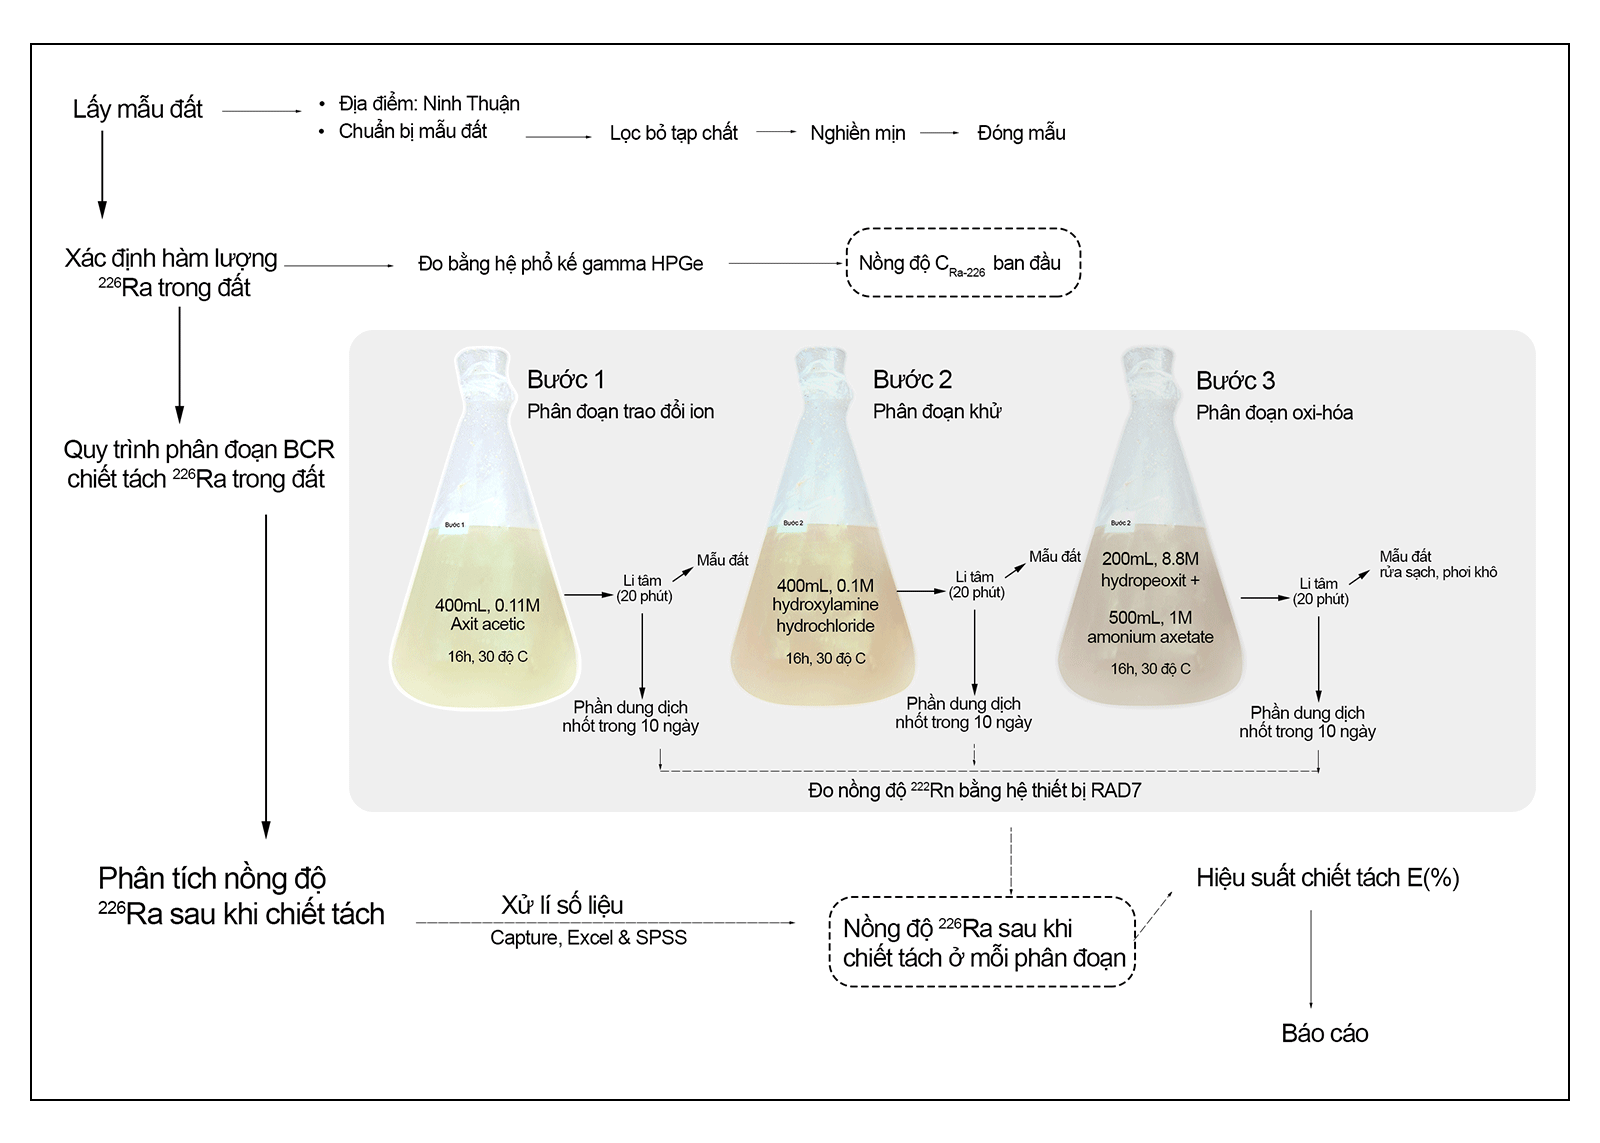
\includegraphics[width=1.1\textwidth]{Image/BCR-Figure1.png}
        \caption{Tóm tắt quy trình xử lí nhiễm bẩn \ce{^226Ra} trong đất}
        \label{figure:DiagramRadiuminSoilBCR}
    \end{figure}


\section{Quy trình lọc tách \ce{^226Ra} trong nước }

\subsection{Xác định nồng độ \ce{^226Ra} trong nước trước khi lọc}
\textbf{Chuẩn bị mẫu}

Các mẫu nước sử dụng cho mục đích nghiên cứu của khóa luận là nước giếng được thu thập tại một số giếng đào thuộc khu vực huyện Ninh Sơn, tỉnh Ninh Thuận. Dùng bộ dụng cụ lấy nước giếng như trong hình ~\ref{figure:EquipmentForMnO2} để lấy mẫu nước giếng. Độ sâu lấy mẫu khoảng 1 m tính từ bề mặt nước. Thể tích mỗi mẫu được lấy là 1 lít.

\begin{figure}[htbp]
    \centering
    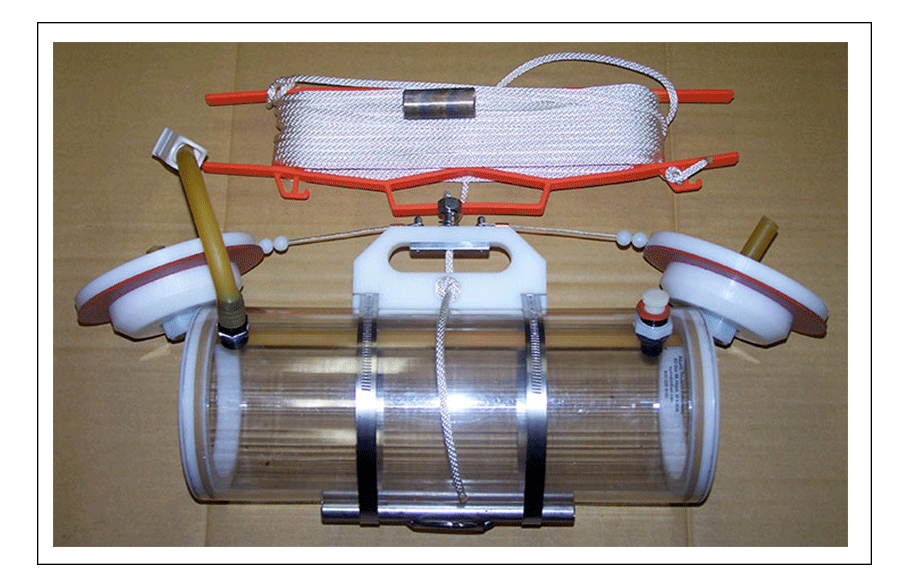
\includegraphics[width=0.8\textwidth]{Image/MnO2-Figure4.png}
    \caption{Dụng cụ lấy mẫu nước}
    \label{figure:EquipmentForMnO2}
\end{figure}

Mẫu sau khi lấy được đo đạc nhanh tại hiện trường một số thông số hóa lý như: nhiệt độ, độ pH. Mỗi mẫu nước sau khi chuyển về phòng thí nghiệm được lấy 250 ml để định lượng \ce{^226Ra}. 

\textbf{Xác định nồng độ \ce{^226Ra} trong nước bằng hệ thiết bị RAD7} 


Mỗi lọ 250 ml nước giếng được khử sạch radon bằng cách bơm đẩy khí ra ngoài lọ. Sau đó, lọ chứa nước giếng được nhốt kín khoảng 10 ngày trước khi xác định nồng độ \ce{^226Ra}. Nồng độ \ce{^226Ra} được xác định thông qua nồng độ radon. Quy trình xác định nồng độ \ce{^226Ra} trong các mẫu nước giếng được trình bày chi tiết trong phần hệ thiết bị RAD7.  

 

 
\subsection{Quy trình điều chế sợi tổng hợp tẩm mangan dioxit}
       
\subsubsection{Thiết bị, dụng cụ và hóa chất}
   
    \textbf{Thiết bị}
        \begin{itemize}
            \item Hệ thiết bị RAD7 của hãng Durridge
            \item Cân điện tử tiểu li: Cân 5 số model PR227/E(2018) của công ty OHAUS, Mỹ (Khối lượng phân tích tối đa 200g, độ chính xác 0,01 mg).
            \item Đèn sấy hồng ngoại của Công ty NTE, Việt Nam (2018), công suất 250W
            \item Bút đo pH điện tử pHTestr30 Waterproof của Công ty OAKTON,  Mỹ, phạm vi đo pH từ –1.00 đến 15.00, ở nhiệt độ từ 0 - 50 (độ C).
            
        \end{itemize}

    \textbf{Dụng cụ và vật liệu}
        \begin{itemize}
            \item Nhiệt kế thủy ngân ($0-100 ^\circ C$, sai số $0.1 ^\circ C$)
            \item Đũa thủy tinh (20cm) và muỗng nhôm.
            \item Cốc thủy tinh chia vạch(50mL, 200mL và 500mL), pipet (2mL), micropipet các  loại của hãng DURAN, Đức.
            \item Lọ thủy tinh (250mL, độ chia nhỏ nhất 50mL) của hãng DURAN, Đức.
            \item Phểu lọc sứ và phểu lọc thủy tinh đường kính phểu 75mm của Genlab, Trung Quốc.
            \item Dây truyền dịch chiều dài 50cm của Công ty Vinamed, Việt Nam.
            \item Bộ giá đỡ thí nghiệm.
            \item Vải sợi tổng hợp thành phần: 90\% polyester, còn lại là sợi polyamid và cotton, kích thước 20cm x 50cm của Công ty Đông Châu, Việt Nam.
            \item Bông gòn 100g của công ty Bông Bạch Tuyết, Việt Nam.
            \item Giấy lọc Whatman loại 1 (11 micron) của hãng Whatman, Mỹ.
        \end{itemize}

    \textbf{Hóa chất}
        \begin{itemize}
            \item \ce{KMnO4} (độ tinh khiết 98.5\%) tinh thể loại P.A, khối lượng 500g của hãng Merck, Mỹ.
            \item Silica gel \ce{SiO2} (độ tinh khiết 95\%), dạng bột mịn (0.5-1.5mm), khối lượng 500g của công ty TRỌNG KHANG , Vietnam.
            \item dung dịch \ce{HCl} (36.5\%-300mL) , hydro peroxit (80\%-300mL)  và dung dịch \ce{NH4OH} (30\%-300mL), dung dịch \ce{NaOH} (3M)  của hãng Merck, Mỹ.
        \end{itemize}
        

    \subsubsection{Các bước thực hiện điều chế sợi tổng hợp tẩm \ce{MnO2}}
        \textbf{Chuẩn bị hóa chất và dụng cụ}
        
        \begin{itemize}
            \item  Lấy 24,06g bột \ce{KMnO4} hòa tan trong nước cất với thể tích 270mL để thu được dung dịch \ce{KMnO4} (0,5M, 300mL).
            \item  Ngâm sợi tổng hợp với dung dịch \ce{HCl} (20mL - 5\%), hydro peroxit (10mL-80\%) trong 200mL nước cất, ở nhiệt độ phòng trong thời gian 2h. Thực hiện bước này nhằm loại bỏ hóa chất nhuộm vải, và các nấm móc có trong vải sợi, và nhằm hạn chế thấp nhất các điều kiện bên ngoài tác động đến các liên kết của sợi vải.\\
        \end{itemize}



        \textbf{Bước 1}: Ngâm sợi tổng hợp  polyester trong dung dịch 0,5M \ce{KMnO4} trong 2h ở nhiệt độ khoảng $50 - 65 ^\circ C$, 20g chất nền \ce{SiO2} . \ce{KMnO4} bị oxy hóa tạo thành \ce{MnO2} gắn lên bề mặt sợi acrylic và chất nền \ce{SiO2}. Vấn đề cần lưu ý là trong quá trình phản ứng, cần điều chỉnh và ổn định nhiệt độ dung dịch không vượt quá $ 65 ^\circ C$. Sau 1h, sợi acrylic chuyển dần sang màu cam và cuối cùng chuyển thành màu đen (\ce{MnO2}) (trong hình ~\ref{figure:MauVaiBeforeAfterMnO2}), do \ce{KMnO4} bị oxi hoá phân huỷ nhiệt  tạo thành \ce{MnO2} theo phương trình phản ứng:

        \begin{equation*}
            \ce{2KMnO4 ->[$t^o$] K2MnO4 + MnO2 + O2 ^}
        \end{equation*}

        \begin{figure}[htbp]
            \centering
            \includegraphics[width=0.95\textwidth]{Image/MnO2-Figure6.png}
            \caption{Mẫu vải sợi tổng hợp polyester trước và sau khi tẩm \ce{MnO2}}
            \label{figure:MauVaiBeforeAfterMnO2}
        \end{figure}

         
        \textbf{Bước 2}: Sợi sau khi tẩy được lấy ra, rửa sạch bằng nước cất, lắc nhẹ để loại bỏ \ce{KMnO4} dư và phần \ce{MnO2} chưa được hình thành liên kết với sợi
        
        \textbf{Bước 3:} Thực hiện sấy khô sợi ở $ 80^\circ C$, trong vòng 30 phút.



\subsubsection{Các bước lọc \ce{^226Ra} trong nước bằng sợi tổng hợp tẩm \ce{MnO2}}        
        \textbf{Bước 1} Chuẩn bị

        \begin{itemize}
            \item Phểu lọc được bọc lót cẩn thận với 3 tấm lọc: Lớp lọc trên cùng là vải sợi tẩm \ce{MnO2} độ dày 5mm, phần giữa là bông gòn và giấy lọc, dưới cùng là vải sợi tẩm \ce{MnO2} độ dày 10mm. 
            \item Các dụng cụ lọc được sắp đặt như trong hình ~\ref{figure:QuyTrinhlocMnO2}
            \item Các mẫu nước được lọc thô bằng vải mỏng để loại bỏ cặn. Sau đó, điều chỉnh pH của mẫu nước ở khoảng từ 7-7.5 bằng dung dịch \ce{HCl} (5\%) và \ce{NH4OH} (10\%), theo ~\cite{MnO2:WillardS.Moore} trong khoảng pH trên thì hiệu suất hấp thụ \ce{^226Ra} của \ce{MnO2} là cao và tối ưu. Sau đó, mẫu nước được đựng trong bình lọc ở thể tích 250mL
        \end{itemize}  

        \textbf{Bước 2} Lọc nước
            \begin{itemize}
                \item Thực hiện lọc mẫu nước trong vòng từ 30-45 phút, ở nhiệt độ phòng từ 28-30 (độ C). Lưu ý, phải điều chỉnh tốc độ dòng chảy của nước ổn định ở  2 (mL/phút) và nhiệt độ ổn định, hạn chế tác động ngoại lực từ bên ngoài lên phểu lọc để nước thấm đều tấm lọc, và hạn chế nước tràn ra ngoài. Hình ~\ref{figure:MnO2SoDoLoc}, thể hiện sơ đồ bố trí thiết bị - dụng cụ lọc mẫu nước bằng sợi tổng hợp tẩm \ce{MnO2}. 
                \item Nước sau khi lọc được đựng trong lọ thủy tinh 250mL và nhốt trong vòng 10 ngày, sau đó thực hiện đo trên hệ thiết bị RAD7.
            \end{itemize}


        \textbf{Bước 3} Đo mẫu phân tích:
         Mẫu nước sau khi được nhốt trong vòng 10 ngày, thực hiện đo trên hệ thiết bị RAD7 trong vòng 4-5h. Dữ liệu đo thể hiện trong phần mềm CAPTURE version 5.7 của hãng Durridge.  Mẫu nước sau khi đo được rửa giải bằng dung dịch hydro peroxit và dung dịch \ce{HCl} (35.6\%), cuối cùng được trung hòa bằng dung dịch \ce{NaOH}. 
            
       
        \begin{figure}
            \centering
            \caption{Sơ đồ bố trí thiết bị và dụng cụ lọc mẫu nước }
            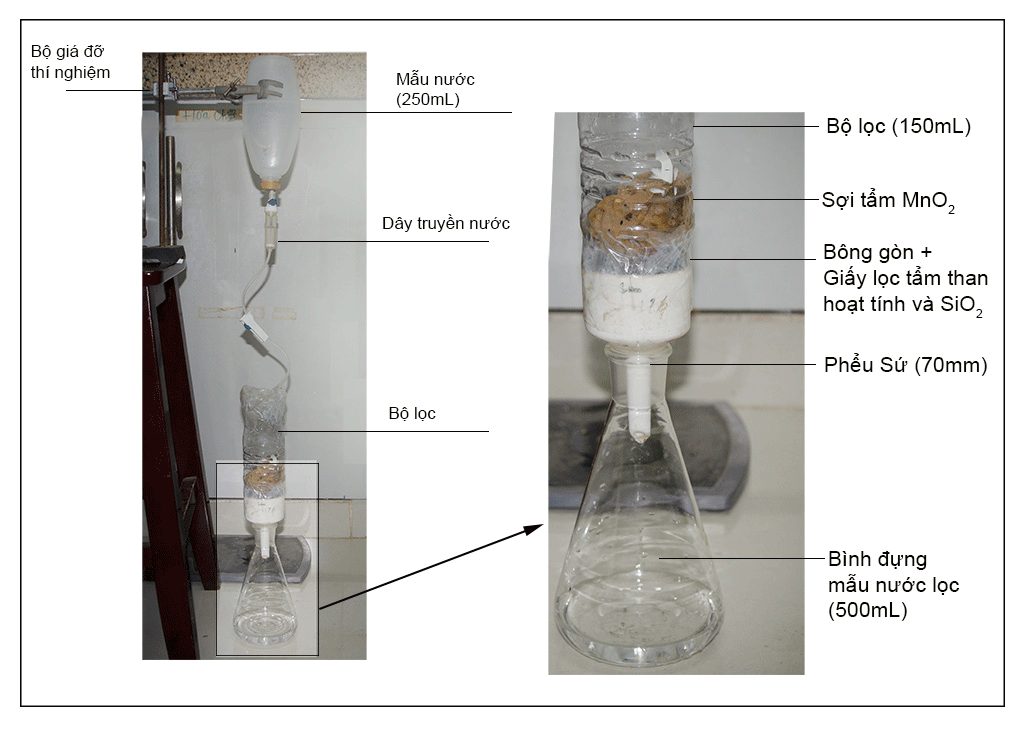
\includegraphics[width=0.85\textwidth]{Image/MnO2-Figure5.png}
            \label{figure:MnO2SoDoLoc}
        \end{figure}


    \subsubsection{Phân tích nồng độ \ce{^226Ra} sau khi lọc tách bằng sợi tổng hợp tẩm \ce{MnO2}}

         \textbf{Hiệu suất quy trình lọc \ce{^226Ra}} :
         
         Hiệu suất quy trình lọc tách \ce{226Ra} trong mẫu nước bằng  sợi tổng hợp \ce{MnO2} được tính theo công thức: 
            \begin{equation}
                E (\%) = \qty(1 - \dfrac{C_2}{C_1}).100\%
            \end{equation}

           Sai số phần trăm hấp thụ 
           \begin{equation}
            \sigma_E = \qty(\dfrac{C_2}{C_1}).\sqrt{\qty(\dfrac{\sigma_{C_1}}{C_1})^2+\qty(\dfrac{\sigma_{C_2}}{C_2})^2}
        \end{equation}

        Trong đó: 
        \begin{itemize}
            \item $C_1 \pm \sigma_{C_1}(Bq/m^3)$: Nồng độ \ce{^226Ra} trong mẫu nước trước khi lọc hấp thụ.  
            \item $C_2  \pm \sigma_{C_2} (Bq/m^3)$: Nồng độ \ce{^226Ra} trong mẫu nước sau khi lọc hấp thụ bằng sợi \ce{MnO2}.
        \end{itemize}
 


    \textbf{ Liều hiệu dụng hằng năm do uống nước chứa \ce{^222Rn}  và \ce{^226Ra}}

      Liều hiệu dụng hằng năm $D_w$ (Sv) mà một người nhận được từ uống nước chứa đồng vị \ce{^222Rn} và \ce{^226Ra} và sai số được tính toán theo công thức:  
      \begin{align}
          &D_w = \varepsilon. V. C_w\\
          &\sigma_{D_w} = \varepsilon.V.\sigma_{C_w} \varepsilon = \dfrac{E}{C}.\sigma_{C_w}
      \end{align}
      Trong đó: 
      \begin{itemize}
          \item $\varepsilon$ là hệ số chuyển đổi liều hiệu dụng trên một đơn vị nồng độ phóng xạ, với \ce{^222Rn}: giá trị $\varepsilon= 10^{-8}$ (Sv/Bq), trong trường hợp \ce{^226Ra} thì giá trị $\varepsilon  = 2,8 \times 10^{-7} $ (Sv/Bq)
          \item $C_w \pm \sigma_{C_w}  (Bq/m^3)  $ là nồng độ tuyệt đối của  \ce{^222Rn}  hoặc \ce{^226Ra}
          \item V là thể tích mỗi người uống trung bình một năm. Từ các số liệu thống kê, trong một ngày một người uống  uống 2 lít nước thì giá trị $V  = 2.10^{-3} \times 365 = 0,73 (m^3) $ 
      \end{itemize}
     Theo báo cáo của UNSCEAR (2000), liều hiệu dụng trung bình toàn cầu do uống nước chứa \ce{^222Rn} khoảng 2 ($\mu Sv$/năm), và nước  chứa \ce{^226Ra} khoảng 8  ($\mu Sv$/năm).  Cơ quan bảo vệ môi trường Hoa Kì, USEPA, đã đưa ra mức giới hạn nồng độ  \ce{^222Rn} và \ce{^226Ra} trong nước lần lượt là 11,1 (Bq/L) và 0,185 (Bq/L) ~\cite{Thesis:HNPThu}. 
     
     
      
     Hình ~\ref{figure:DiagramRadiuminSoilBCR}, mô tả tóm tắt quy trình xử lí nhiễm bẩn \ce{^226Ra} trong nước bằng quy trình hấp thụ \ce{^226Ra} trên sợi tổng hợp tẩm \ce{MnO2}

     \begin{figure}[htbp]
         \centering
         \includegraphics[width=0.85\textwidth]{Image/MnO2-Figure3.png}
         \caption{Tóm tắt quy trình xử lí nhiễm bẩn \ce{^226Ra} trong nước}
         \label{figure:MnO2SoDoTomTat}
     \end{figure}
 
       
 

        
        
        
        